\documentclass{goose-article}

\hypersetup{pdfauthor={T.W.J. de Geus}}

\title{Linear elasticity}

\author[1]{Tom de Geus}

\begin{document}

\maketitle

\section{Constitutive model}

The stress, $\bm{\sigma}$, is set by to the strain, $\bm{\varepsilon}$, through the following linear relation:
\begin{equation}
  \bm{\sigma} \equiv K \mathrm{tr}\left( \bm{\varepsilon} \right) + 2 G \bm{\varepsilon}_\mathrm{d} \equiv \mathbb{C} : \bm{\varepsilon}
\end{equation}
wherein $\mathbb{C}$ is the elastic stiffness, which reads:
\begin{align}
  \mathbb{C}
  &\equiv K \bm{I} \otimes \bm{I}
   + 2 G (\mathbb{I}_\mathrm{s} - \tfrac{1}{3} \bm{I} \otimes \bm{I} )
  \\
  &= K \bm{I} \otimes \bm{I}
  + 2 G \, \mathbb{I}_\mathrm{d}
\end{align}
with $K$ and $G$ the bulk and shear modulus respectively. See Appendix~\ref{sec:ap:nomenclature} for nomenclature, including definitions of the unit tensors.

\section{Consistency check}

To check if the derived tangent $\mathbb{C}$ a \emph{consistency check} can be performed. A (random) perturbation $\delta \bm{\varepsilon}$ is applied. The residual is compared to that predicted by the tangent. For the general case of linearisation, the following holds:
%
\begin{equation}
  \bm{\sigma}\big( \bm{\varepsilon}_\star + \delta \bm{\varepsilon} \big) =
  \bm{\sigma}\big( \bm{\varepsilon}_\star \big) +
  \mathbb{C} \big( \bm{\varepsilon}_\star \big) : \delta \bm{\varepsilon} +
  \mathcal{O}(\delta \bm{\varepsilon}^2)
\end{equation}
%
or
%
\begin{equation}
  \underbrace{
    \bm{\sigma}\big( \bm{\varepsilon}_\star + \delta \bm{\varepsilon} \big) -
    \bm{\sigma}\big( \bm{\varepsilon}_\star \big)
  }_{
    \displaystyle \delta \bm{\sigma}
  } -
  \mathbb{C} \big( \bm{\varepsilon}_\star \big) : \delta \bm{\varepsilon} =
  \mathcal{O}(\delta \bm{\varepsilon}^2)
\end{equation}
%
This allows the introduction of a relative error
%
\begin{equation}
  \eta =
  \Big|\Big|
    \delta \bm{\sigma} -
    \mathbb{C}(\bm{\varepsilon}_\star) : \delta \bm{\varepsilon}
  \Big|\Big|
  /
  \Big|\Big| \delta \bm{\sigma} \Big|\Big|
\end{equation}
%
This \emph{truncation error} thus scales as $\eta \sim || \delta \bm{\varepsilon} ||^2$ as depicted in Figure~\ref{fig:consistency:expected}. As soon as the error becomes sufficiently small the numerical \emph{rounding error} becomes more dominant, the scaling thereof is also included in Figure~\ref{fig:consistency:expected}.

\begin{figure}[htp]
  \centering
  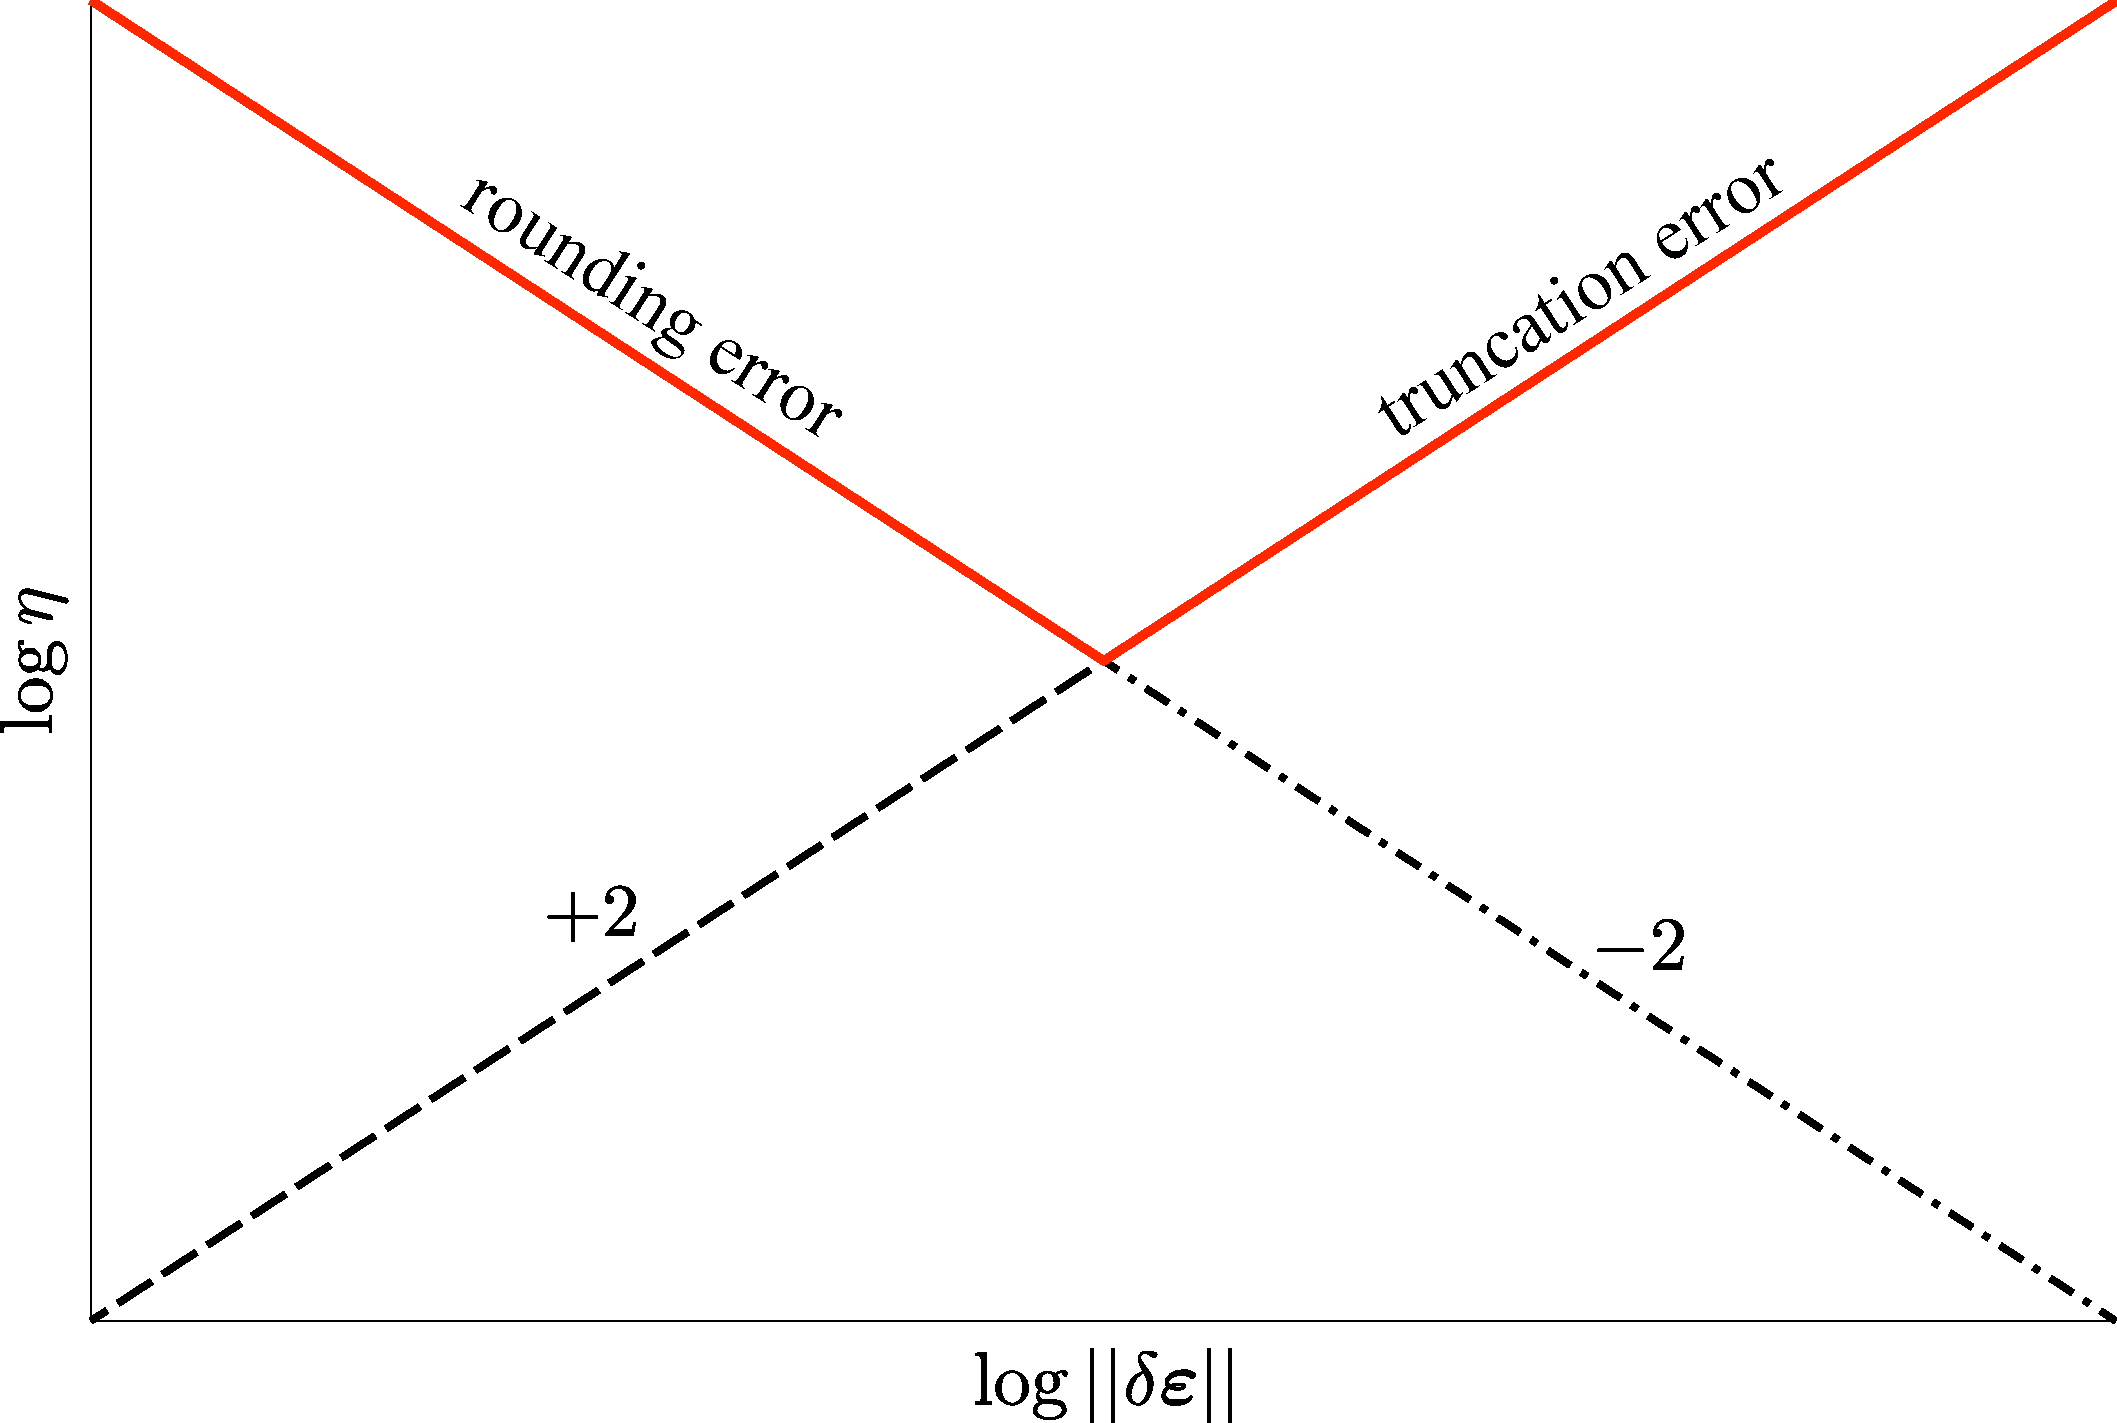
\includegraphics[width=.5\textwidth]{figures/consistency}
  \caption{Expected behaviour of the consistency check, see \citet[p.~9]{Heath2002}.}
  \label{fig:consistency:expected}
\end{figure}

Because this model is linear there is no truncation error, the measurement of $\eta$ and a function of $|| \delta \bm{\varepsilon} ||$ thus only displays a rounding error, as depicted in Fig.~\ref{fig:consistency}.

\begin{figure}[htp]
  \centering
  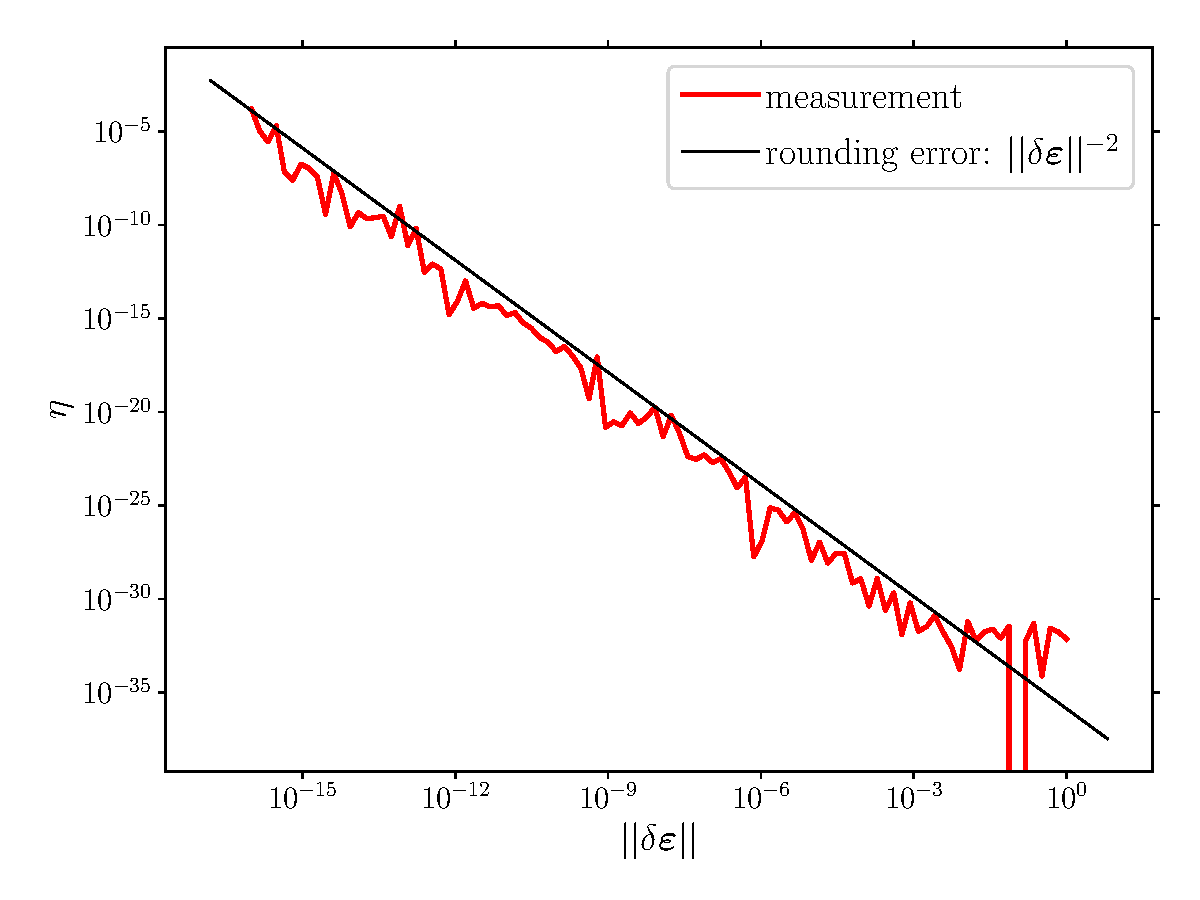
\includegraphics[width=.5\textwidth]{examples/consistency}
  \caption{Measured consistency check, cf.\ Fig.~\ref{fig:consistency:expected}.}
  \label{fig:consistency}
\end{figure}

\appendix

\section{Nomenclature}
\label{sec:ap:nomenclature}

\paragraph{Tensor products}
\vspace*{.5eM}

\begin{itemize}
%
\item Dyadic tensor product
\begin{align}
  \mathbb{C} &= \bm{A} \otimes \bm{B} \\
  C_{ijkl}   &= A_{ij} \,      B_{kl}
\end{align}
%
\item Double tensor contraction
\begin{align}
  C &= \bm{A} : \bm{B} \\
    &= A_{ij} \, B_{ji}
\end{align}
%
\end{itemize}

\paragraph{Tensor decomposition}
\vspace*{.5eM}

\begin{itemize}
%
\item Deviatoric part $\bm{A}_\mathrm{d}$ of an arbitrary tensor $\bm{A}$:
\begin{equation}
  \mathrm{tr}\left( \bm{A}_\mathrm{d} \right) \equiv 0
\end{equation}
and thus
\begin{equation}
  \bm{A}_\mathrm{d} = \bm{A} - \tfrac{1}{3} \mathrm{tr}\left( \bm{A} \right)
\end{equation}
%
\end{itemize}

\paragraph{Fourth order unit tensors}
\vspace*{.5eM}

\begin{itemize}
%
\item Unit tensor:
\begin{equation}
  \bm{A} \equiv \mathbb{I} : \bm{A}
\end{equation}
and thus
\begin{equation}
  \mathbb{I} = \delta_{il} \delta{jk}
\end{equation}
%
\item Right-transposition tensor:
\begin{equation}
  \bm{A}^T \equiv \mathbb{I}^{RT} : \bm{A} = \bm{A} : \mathbb{I}^{RT}
\end{equation}
and thus
\begin{equation}
  \mathbb{I}^{RT} = \delta_{ik} \delta_{jl}
\end{equation}
%
\item Symmetrisation tensor:
\begin{equation}
  \mathrm{sym} \left( \bm{A} \right) \equiv \mathbb{I}_\mathrm{s} : \bm{A}
\end{equation}
whereby
\begin{equation}
  \mathbb{I}_\mathrm{s} = \tfrac{1}{2} \left( \mathbb{I} + \mathbb{I}^{RT} \right)
\end{equation}
This follows from the following derivation:
\begin{align}
  \mathrm{sym} \left( \bm{A} \right) &= \tfrac{1}{2} \left( \bm{A} + \bm{A}^T \right)
  \\
  &= \tfrac{1}{2} \left( \mathbb{I} : \bm{A} + \mathbb{I}^{RT} : \bm{A} \right)
  \\
  &= \tfrac{1}{2} \left( \mathbb{I} + \mathbb{I}^{RT} \right) : \bm{A}
  \\
  &= \mathbb{I}_\mathrm{s} : \bm{A}
\end{align}
%
\item Deviatoric and symmetric projection tensor
\begin{equation}
  \mathrm{dev} \left( \mathrm{sym} \left( \bm{A} \right) \right) \equiv \mathbb{I}_\mathrm{d} : \bm{A}
\end{equation}
from which it follows that:
\begin{equation}
  \mathbb{I}_\mathrm{d}
  = \mathbb{I}_\mathrm{s} - \tfrac{1}{3} \bm{I} \otimes \bm{I}
\end{equation}
%
\end{itemize}

\bibliography{library}

\end{document}
